\documentclass[12pt]{article}

% font
\usepackage{lmodern}

% packages
\usepackage[margin=1in, a4paper]{geometry}
\usepackage{indentfirst}
\usepackage{amsmath}
\usepackage{mathtools}
\usepackage{sectsty}
\usepackage{footmisc}
\usepackage{gensymb}
\usepackage{xcolor}
\usepackage{listings}
\usepackage{caption}
\usepackage[colorlinks, allcolors=blue]{hyperref}
\usepackage[scaled=0.9]{DejaVuSansMono}

% size config of sections
\sectionfont{\fontsize{12}{15}\selectfont}
\subsectionfont{\fontsize{12}{15}\selectfont}
\subsubsectionfont{\fontsize{12}{15}\selectfont}

% basic config
\setlength\parindent{24pt}
\renewcommand{\thefootnote}{\fnsymbol{footnote}}
\sloppy

% lst listings config
\definecolor{codegreen}{rgb}{0,0.6,0}
\definecolor{codegray}{rgb}{0.5,0.5,0.5}
\definecolor{codepurple}{rgb}{0.58,0,0.82}
\definecolor{backcolour}{rgb}{0.95,0.95,0.92}

\lstdefinestyle{lstlistings_stylesheet}{
    backgroundcolor=\color{backcolour},
    commentstyle=\color{codegreen},
    keywordstyle=\color{magenta},
    numberstyle=\tiny\color{codegray},
    stringstyle=\color{codepurple},
    basicstyle=\ttfamily\scriptsize,
    breakatwhitespace=false,
    breaklines=true,
    captionpos=b,
    keepspaces=true,
    numbers=left,
    numbersep=5pt,
    showspaces=false,
    showstringspaces=false,
    showtabs=false,
    tabsize=4
}
\lstset{style=lstlistings_stylesheet}

% paper info
\title{helloworld}
\author{John Doe}
\date{August 13, 2022}

\begin{document}
	
	\section{This is a section: Math}
	
	This program is planned to support the most basic LaTeX features, you can use inline math with $a + b = c^2$. And this will be the paragraph math:
	
	\begin{equation}
		\oint \boldsymbol{B} \cdot d \boldsymbol{A} = 0
	\end{equation}
	
	And this is for align:
	
	\begin{align}
		\sum_{i} \vec{B_{i}} \cdot \vec{\ell_{i}} &= \mu_{0} \bigg(I + \varepsilon_{0} \frac{\Delta E \cdot A}{\Delta t} \bigg)\\
		\sum_{i} \vec{E_{i}} \cdot \vec{\ell_{i}} &= - \frac{\Delta B \cdot A}{\Delta t}\\
		\sum_{i} E_{i} \cdot A_{i} &= \frac{Q}{\varepsilon_{0}}\\
		\sum_{i} B_{i} \cdot A_{i} &= 0
	\end{align}
	
	\subsection{This is subsection: Images}
	
	You can also insert images with:
	
	\begin{figure}[h]
		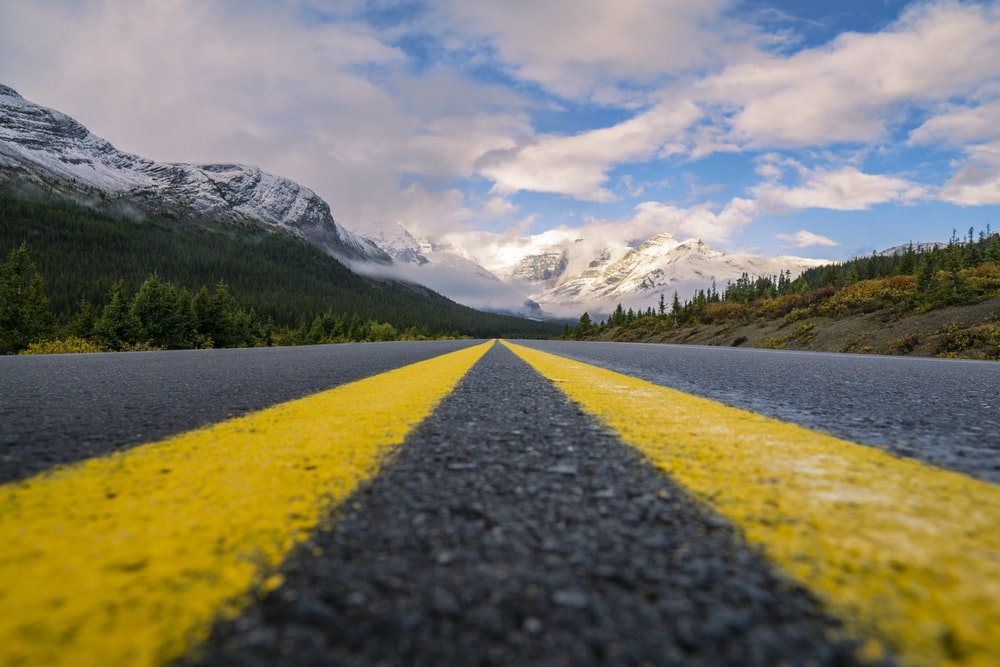
\includegraphics[width=\textwidth]{./sample_image.jpeg}
		\caption{figure}
	\end{figure}
	
	or by:
	
	
	<img src="./sample\_image.jpeg" align="center">
	
	
	\subsubsection{This is subsubsection: Listings}
	
	And code blocks with:
	
	
\begin{lstlisting}[language=c]
#include <stdio.h>


void say() {
    printf("this is code blocks!");
}


int main() {
    char hello_world[] = "hello world!\n";
    printf(helloworld);

    say();

    return 0;
}
\end{lstlisting}
	
	\paragraph{This is paragraph}
	
	Check \href{example.tex}{./example.tex} for the LaTeX rendition of this markdown file. The output of the command is always placed in \texttt{./out/}.
	
\end{document}